\begin{center}
\begin{minipage}[t]{.46\linewidth}\vspace{0pt}\centering
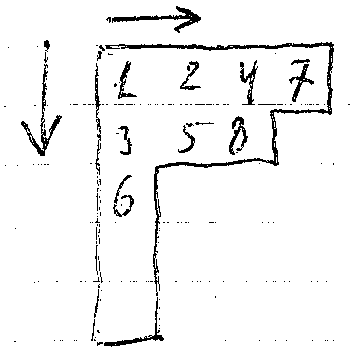
\includegraphics[width=\linewidth]{figures/gelfand-0153-p001414-young-tableau-original.png}\par\smallskip
{\footnotesize Оригинал рукописного рисунка: \texttt{GELFAND-P001414}}
\end{minipage}\hfill
\begin{minipage}[t]{.50\linewidth}\vspace{0pt}\centering
{\footnotesize Частичное воссоздание видимых штрихов}\par\smallskip
\resizebox{\linewidth}{!}{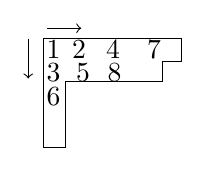
\begin{tikzpicture}[x=0.44cm,y=0.44cm]
\draw (0,0)--(4,0)--(4,-0.65)--(3.45,-0.65)--(3.45,-1.25)--(0.65,-1.25)--(0.65,-3.15)--(0,-3.15)--cycle;
\node at (0.30,-0.33) {$1$};
\node at (1.04,-0.33) {$2$};
\node at (2.02,-0.33) {$4$};
\node at (3.20,-0.33) {$7$};
\node at (0.30,-0.97) {$3$};
\node at (1.15,-0.97) {$5$};
\node at (2.06,-0.97) {$8$};
\node at (0.30,-1.66) {$6$};
\draw[->] (0.12,0.30)--(1.10,0.30);
\draw[->] (-0.43,0.0)--(-0.43,-1.15);
\end{tikzpicture}
}
\end{minipage}
\end{center}
\noindent{\small\textit{Сохранены неровный контур и восемь видимых чисел. Пустая длинная ножка не заполнена; внутренняя сетка клеток не добавлена.}}
